\chapter{Analisi dei Requisiti}
\label{cha:intro}

\textcolor{red}{Lorem ipsum dolor sit amet, consectetur adipiscing elit. Donec sed nunc orci. Aliquam nec nisl vitae sapien pulvinar dictum quis non urna. Suspendisse at dui a erat aliquam vestibulum. Quisque ultrices pellentesque pellentesque. Pellentesque egestas quam sed blandit tempus. Sed congue nec risus posuere euismod. Maecenas ut lacus id mauris sagittis egestas a eu dui.}




\section{Requisiti funzionali}
\label{sec:funzionali}
I requisiti funzionali definiscono le funzioni del sistema, ovvero ciò che questo deve fare in termini di interazione tra l'applicativo e il suo ambiente, indipendentemente dall'implementazione. Questi tipi di requisiti possono essere rappresentati dai casi d'uso, sequenza di azioni che producono un risultato osservabile da un attore, esplicitando cosa ci si aspetta dal sistema ma nascondendone il comportamento.\\
Di seguito si riporta l'elenco dei principali requisiti funzionali individuati con una breve descrizione. Si nota che l'analisi relativa alle anagrafiche è riportata ad alto livello raggruppandole sotto un unico componente.
\subsection{Accesso protetto al sistema}
\textbf{Riassunto}: si descrive come avviene l'autenticazione di un utente che vuole accedere al gestionale.\\
\textbf{Descrizione:}
\begin{enumerate}
  \item L'utente non autenticato inserisce username e password per accedere.
  \item Il sistema verifica la correttezza dei dati inseriti interrogando il database.
  \item Se l'interrogazione ha esisto positivo l'utente autenticato accede alla homepage, altrimenti il sistema segnala la non correttezza dei dati.
\end{enumerate}

\subsection{Visualizzazione delle anagrafiche}
\textbf{Riassunto}: si descrive come il sistema mostra i dati relativi alle varie anagrafiche.\\
\textbf{Descrizione:}
\begin{enumerate}
  \item Il sistema presenta i dati dell'anagrafica selezionata in forma tabellare e strutturata.
  \item L'utente naviga nella tabella con la possibilità di filtrare o navigare tra i dati.
  \item Il sistema risponde alle richieste dell'utente adattando la visualizzazione di conseguenza.
\end{enumerate}

\subsection{Memorizzazione delle anagrafiche}
\textbf{Riassunto}: si descrive come il sistema garantisce la memorizzazione di nuovi dati relativi alle anagrafiche.\\
\textbf{Descrizione:}
\begin{enumerate}
  \item L'utente aggiunge nuovi elementi alle anagrafiche inserendo i dati richiesti dal sistema.
  \item Il sistema verifica la correttezza e la completezza dei dati inseriti. Se la verifica ha esito positivo prosegue altrimenti segnala l'errore.
  \item Il sistema memorizza nel database il nuovo elemento.
  \item Il sistema aggiorna la visualizzazione dei dati.
\end{enumerate}

\subsection{Gestione delle anagrafiche}
\textbf{Riassunto}: si descrive come l'utente accede alle funzionalità dei dati relativi alle anagrafiche.\\
\textbf{Descrizione:}
\begin{enumerate}
  \item L'utente seleziona un elemento di un'anagrafica.
  \item Se l'utente sceglie di modificare un elemento:
  \begin{enumerate}
    \item Il sistema verifica la correttezza e la completezza dei nuovi dati. Se la verifica ha esito positivo prosegue altrimenti segnala l'errore.
    \item Il sistema aggiorna l'elemento nel database.
    \item Il sistema aggiorna la visualizzazione dei dati.
  \end{enumerate}
  \item Se l'utente sceglie di eliminare un elemento:
  \begin{enumerate}
    \item Il sistema verifica la possibilità di eliminare l'elemento in termini di non violazione di vincoli con altri elementi. Se la verifica ha esito positivo prosegue altrimenti segnala l'errore.
    \item Il sistema elimina l'elemento dal database.
    \item Il sistema aggiorna la visualizzazione dei dati.
  \end{enumerate}
\end{enumerate}

\subsection{Logout dal sistema}
\textbf{Riassunto}: si descrive come l'utente esce dal sistema.\\
\textbf{Descrizione:}
\begin{enumerate}
  \item L'utente autenticato effettua il logout.
  \item Il sistema termina la sessione dell'utente, che viene scollegato.
\end{enumerate}



\section{Requisiti non funzionali}
\label{sec:nonfunzionali}
I requisiti non funzionali rappresentano i vincoli che il sistema deve soddisfare nella sua totalità. Questi requisiti non sono legati a singole funzioni fornite dal software ma a caratteristiche che questo deve avere in termini di qualità del sistema o vincoli a cui deve sottostare.\\
Di seguito di riporta un elenco dei principali requisiti non funzionali raccolti, con una breve descrizione corrispondente.

\subsection{Responsive web design}
L'applicativo deve essere in grado di adattarsi graficamente in maniera automatica e fluida a qualsiasi dispositivo utilizzato. Il gestionale riconosce quindi il dispositivo utilizzato dall’utente e adatta il suo layout alle specifiche dimensioni del display.

\subsection{Sicurezza}
Il sistema protegge il contenuto da accessi non autorizzati e prevede delle norme di sicurezza in termini di:
\begin{itemize}
  \item Conferma di identità: all'utente non autenticato viene mostrata la pagina di login e, solo dopo il corretto inserimento dei dati con verifica tramite interrogazione al database, potrà accedere al gestionale. 
  \item Sicurezza di trasmissione dei dati: il sistema adotta le tecniche per preservare la riservatezza, l'integrità e la disponibilità dei dati trasmessi ed elaborati anche e soprattutto, tramite l'utilizzo del protocollo \texttt{https}.\cite{https}
  \item Sicurezza delle password: la memorizzazione delle password nel database avviene in maniera criptata; la creazione di una nuova password per l'utente prevede dei vincoli di robustezza e sicurezza quali: lunghezza di almeno 10 caratteri, presenza di almeno 2 lettere maiuscole, 2 simboli e 4 numeri.
\end{itemize}

\subsection{Affidabilità}
Il sistema deve rispettare le specifiche tecniche di funzionamento nel tempo.\cite{affidabilità}
Per garantire tale requisito sono stati imposti dei vincoli di affidabilità:

\begin{table}[h!]
\centering
\begin{tabular}{|l|l|l|}
\hline
\multicolumn{1}{|c|}{\textbf{Vincolo}} & \multicolumn{1}{c|}{\textbf{Descrizione}} & \multicolumn{1}{c|}{\textbf{Misura}} \\ \hline
Tempo di attesa                        & Tempo massimo di risposta alla richiesta  & ≤ 1,5 secondi                        \\ \hline
Tasso di fallimento                    & Risposta a ogni richiesta inviata         & ≤ 0,5\%                              \\ \hline
Tentativo di recupero                  & Riprovare la richiesta fallita            & 5 volte a intervalli di 2 secondi    \\ \hline
\end{tabular}
\caption{Tabella dei vincoli di affidabilità.}
\label{}
\end{table}

\subsection{Usabilità}
Gli utenti devono essere facilmente in grado di navigare tra le risorse e portare a termine le operazioni previste, il sistema deve quindi essere, nella sua integrità, semplice da usare ed efficiente. 

\subsection{Prestazioni}
Il gestionale deve essere veloce in fase di avvio e fluido sia durante la transizione da una pagina all'altra, che durante il caricamento, la visualizzazione dei dati e lo svolgimento di ogni operazione.
Per garantire tale requisito sono stati imposti dei vincoli di performance:
\begin{table}[h!]
\centering
\begin{tabular}{|l|l|l|}
\hline
\multicolumn{1}{|c|}{\textbf{Vincolo}} & \multicolumn{1}{c|}{\textbf{Misura}} \\ \hline
Avvio della pagina principale &  Entro 1 secondo\\ \hline
Transizione tra pagine & Entro 1 secondo\\ \hline
Caricamento dei dati & Entro 3 secondi\\ \hline
Operazione sui dati & Entro 3 secondi\\ \hline
\end{tabular}
\caption{Tabella dei vincoli di performance.}
\label{}
\end{table}

Il sistema deve inoltre gestire l'accesso contemporaneo di più utenti senza alcun degrado delle prestazioni.

\subsection{Scalabilità}
Il sistema riesce a gestire un numero crescente di utenti che accede al gestionale in simultanea e gestisce i dati prodotti dagli utenti stessi.     
Il sistema deve essere anche in grado di aumentare o diminuire in termini di utenti e dati contenuti in base alle esigenze.

\subsection{Compatibilità e Portabilità}
L'applicativo non necessita di installazione all'interno del sistema operativo su cui viene eseguito, la sua compatibilità e portabilità sono quindi strettamente legate al browser utilizzato. Il sistema deve garantire quindi di essere compatibile con i browser più popolari \cite{browsers} come:
\begin{itemize}
  \item Google Chrome, dalla versione 3.22.24.10 \cite{chrome}.
  \item Mozilla Firefox, dalla versione 27 \cite{firefox}.
  \item Safari, dalla versione 8.0 \cite{safari}.
  \item Microsoft Edge, dalla versione 0.11.10051 \cite{edge}.
\end{itemize}
e altri.



\subsection{Manutenzione}
Dopo il rilascio del sistema, deve essere possibile in modo semplice ed efficace eliminare malfunzionamenti, migliorare le prestazione e inserire nuove funzionalità con aggiornamenti.

\section{Analisi delle attività}
\label{sec:contesto}
La fase di analisi delle attività ha come obiettivo la modellazione del flusso di lavoro dell'intero sistema che viene visto come un insieme di azioni che seguendo un processo.\\
Lo schema prodotto crea un grafo diretto in cui ogni nodo descrive un'attività e ogni arco il percorso possibile.  

\subsection{Diagramma delle attività}
\begin{figure}[h]
\centering
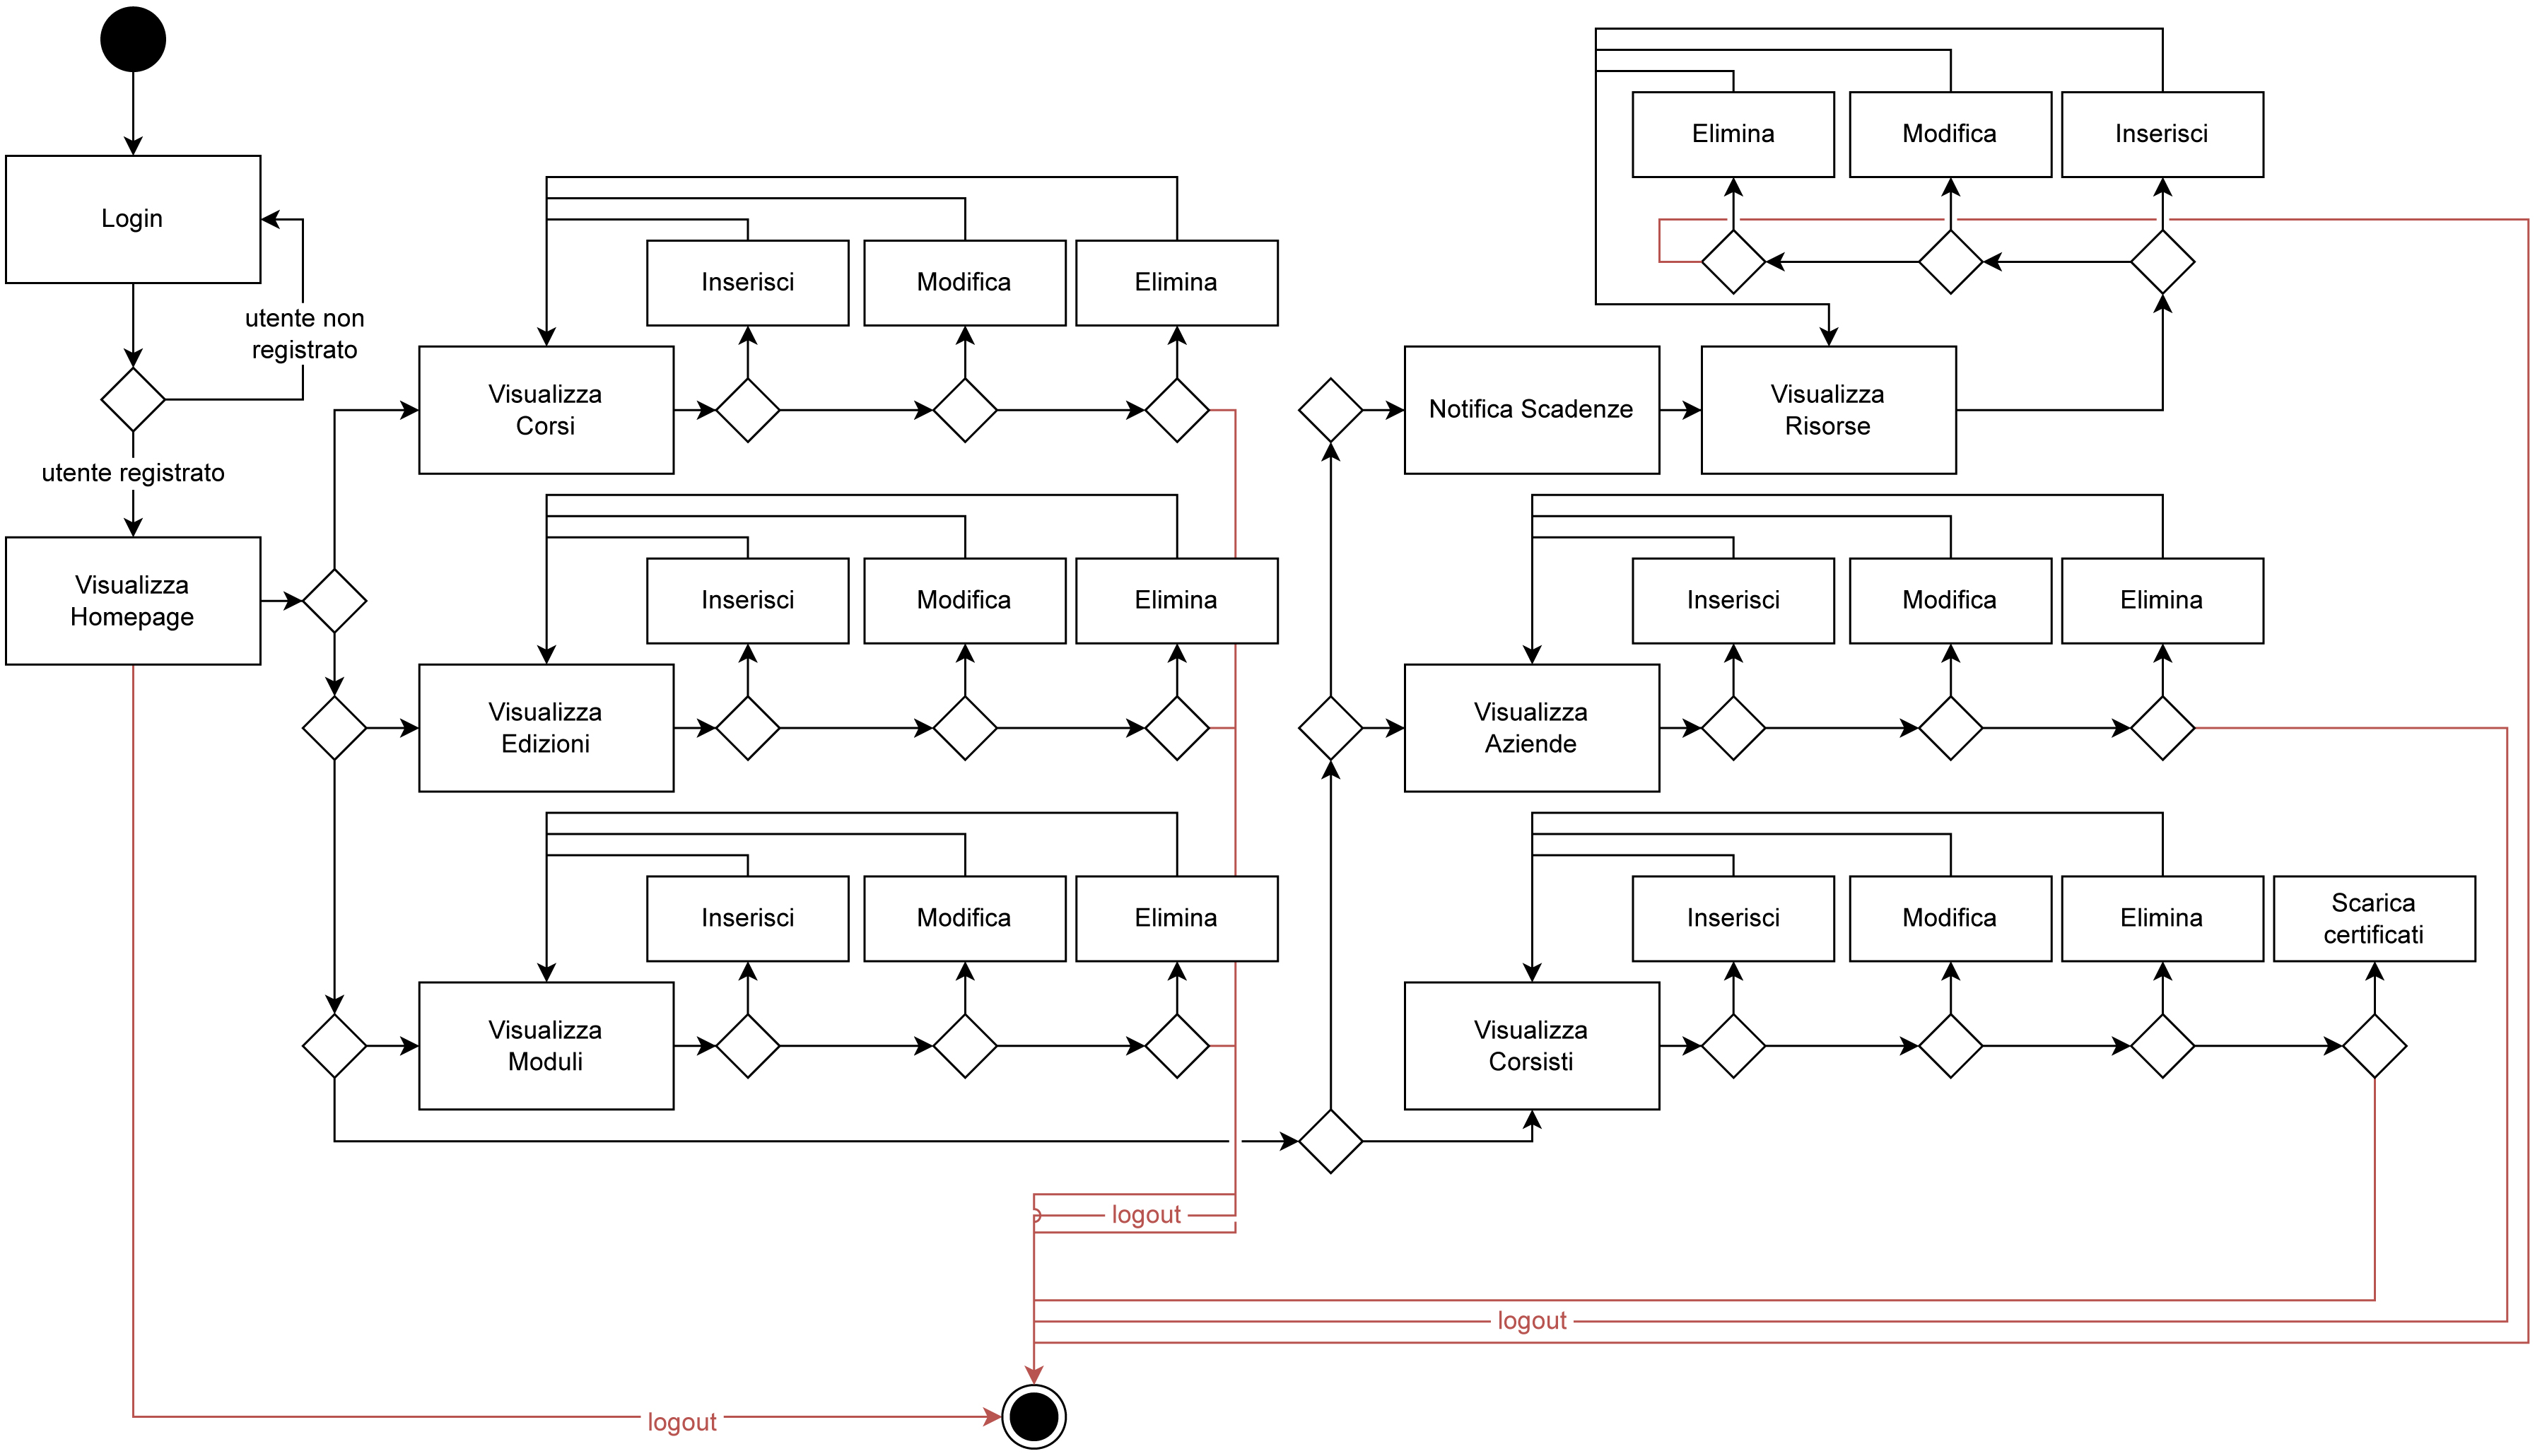
\includegraphics[scale=0.55]{img/Diagramma delle attivita.jpg}
\caption{Diagramma delle attività}
\label{fig:Diagrammadelleattivita}
\end{figure}
\noindent
Il diagramma in figura \ref{fig:Diagrammadelleattivita} rappresenta il diagramma delle attività per l'utente che opera con il sistema che, una volta autenticato, accede a tutte le funzionalità del gestionale.\\
Ogni rettangolo identifica un nodo del grafo o come azione (ad esempio \textit{Visualizza Corsi}) o come nodo di controllo (come \textit{Logout}); i rombi sono invece nodi di decisione per coprire tutti i possibili percorsi tra le attività.



\section{Analisi del contesto}
\label{sec:contesto}
L'analisi del contesto è quella fase in cui si prendono in considerazione le iterazione che il software ha con gli altri sistemi in relazione al flusso di informazioni.

\subsection{Diagramma di contesto}
\begin{figure}[h]
\centering
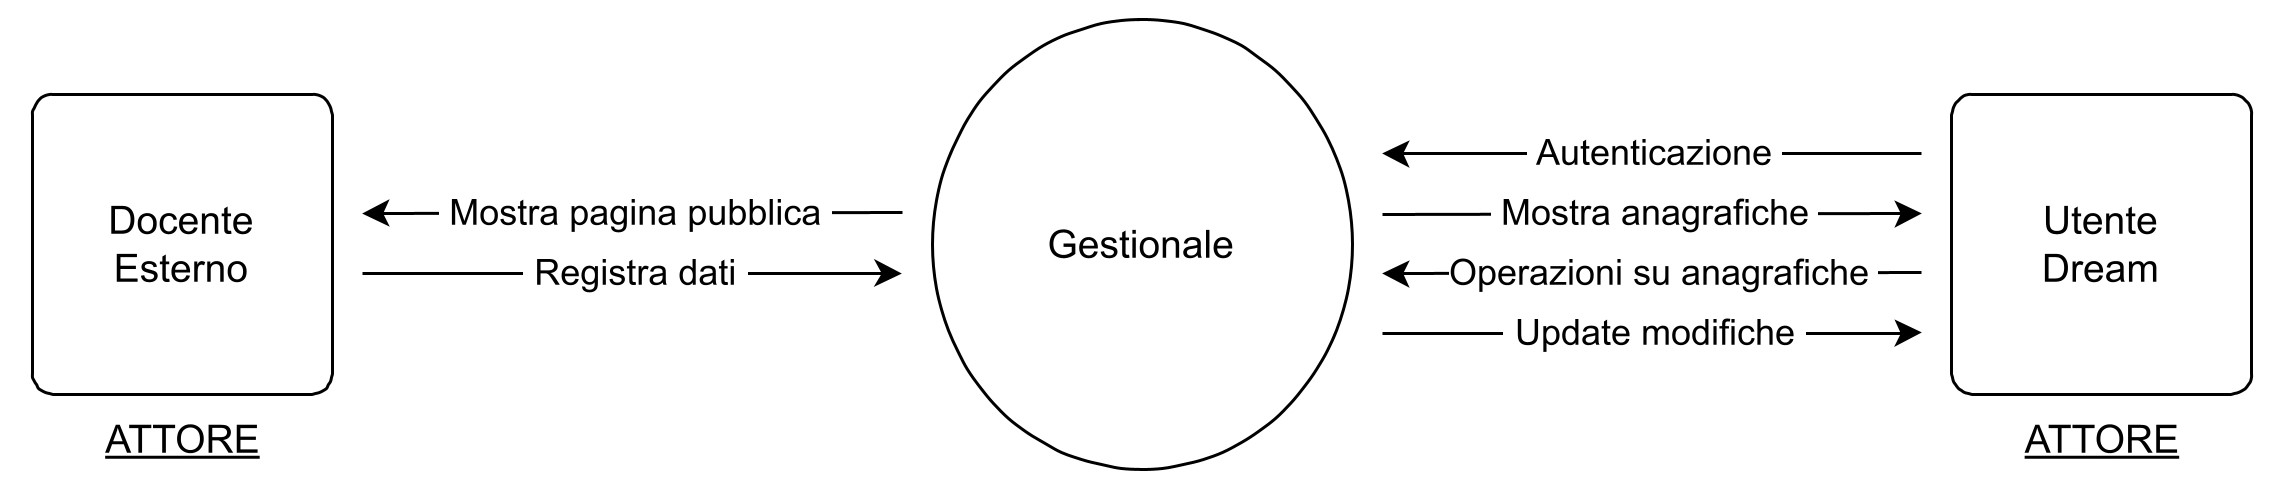
\includegraphics[scale=0.8]{img/Diagramma di Contesto.jpg}
\caption{Diagramma di contesto}
\label{fig:Diagrammadicontesto}
\end{figure}
\noindent
Il diagramma in figura \ref{fig:Diagrammadicontesto} rappresenta le interfacce esterne con cui il gestionale comunica. Si individuano due attori (entità che producono o consumano informazioni necessarie per l’elaborazione delle richieste): \textit{Utente Dream} e \textit{Docente Esterno}, il primo rappresenta l'utente che all'interno dell'azienda utilizza il gestionale mentre il secondo identica un docente che accede alla pagina pubblica per la registrazione a sistema dei suoi dati. Le frecce nel diagramma mostrano i flussi di informazioni.

\section{Analisi dei componenti}
\label{sec:componenti}
Questa fase di analisi ha l'obiettivo di modellare le connessioni tra i componenti, intesi come singoli moduli del software, in modo da evidenziare le relazioni tra essi e verificare che tutti i compiti che il sistema deve svolgere siano implementati. 
\subsection{Diagramma dei componenti}
\begin{figure}[h]
\centering
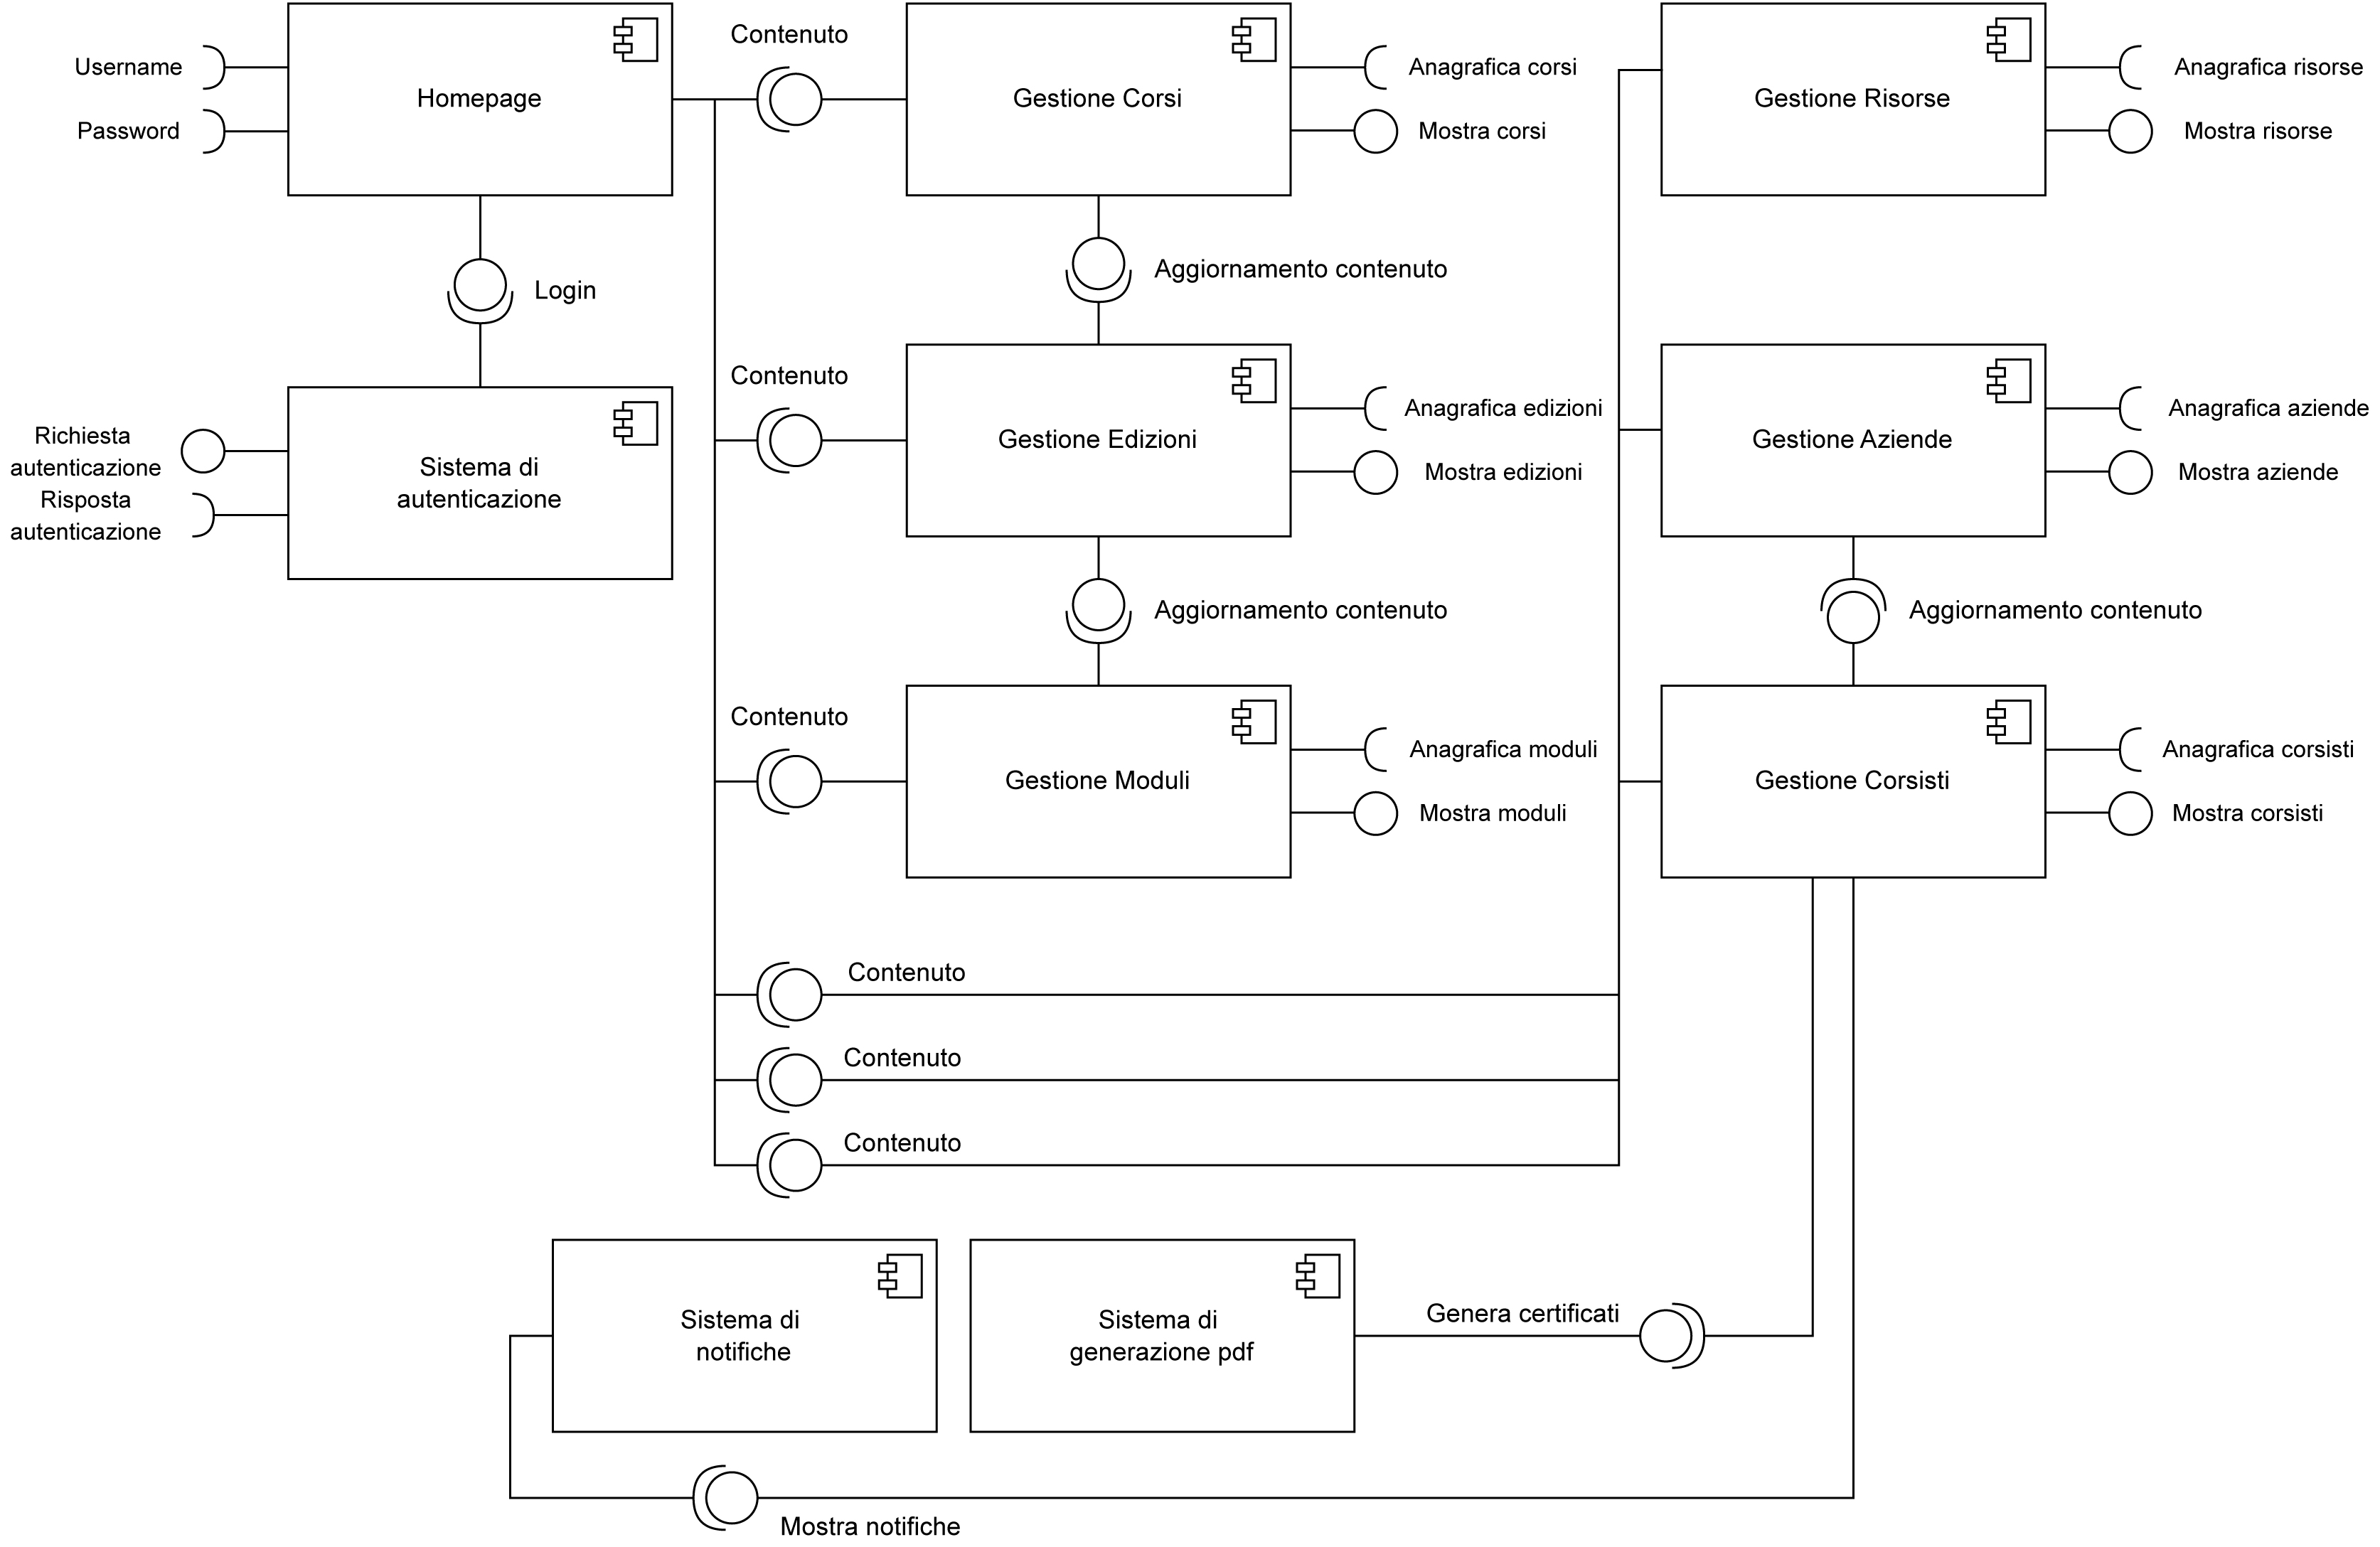
\includegraphics[scale=0.55]{img/Diagramma dei componenti.jpg}
\caption{Diagramma dei componenti}
\label{fig:Diagrammadeicomponenti}
\end{figure}
\noindent
In figura \ref{fig:Diagrammadicontesto} i rettangoli mappano i componenti mentre le relazioni tra due componenti individuano le interfacce. Le relazioni presentano un semicerchio se l'interfaccia è richiesta da un componente che ne consuma le informazioni, se, invece, sono rappresentate con un cerchio allora l'interfaccia in questione è messa a disposizione del componente che ne produce le informazioni.